\documentclass[]{article}
\usepackage{lmodern}
\usepackage{amssymb,amsmath}
\usepackage{ifxetex,ifluatex}
\usepackage{fixltx2e} % provides \textsubscript
\ifnum 0\ifxetex 1\fi\ifluatex 1\fi=0 % if pdftex
  \usepackage[T1]{fontenc}
  \usepackage[utf8]{inputenc}
\else % if luatex or xelatex
  \ifxetex
    \usepackage{mathspec}
    \usepackage{xltxtra,xunicode}
  \else
    \usepackage{fontspec}
  \fi
  \defaultfontfeatures{Mapping=tex-text,Scale=MatchLowercase}
  \newcommand{\euro}{€}
\fi
% use upquote if available, for straight quotes in verbatim environments
\IfFileExists{upquote.sty}{\usepackage{upquote}}{}
% use microtype if available
\IfFileExists{microtype.sty}{%
\usepackage{microtype}
\UseMicrotypeSet[protrusion]{basicmath} % disable protrusion for tt fonts
}{}
\usepackage[margin=1in]{geometry}
\usepackage{longtable,booktabs}
\usepackage{graphicx}
\makeatletter
\def\maxwidth{\ifdim\Gin@nat@width>\linewidth\linewidth\else\Gin@nat@width\fi}
\def\maxheight{\ifdim\Gin@nat@height>\textheight\textheight\else\Gin@nat@height\fi}
\makeatother
% Scale images if necessary, so that they will not overflow the page
% margins by default, and it is still possible to overwrite the defaults
% using explicit options in \includegraphics[width, height, ...]{}
\setkeys{Gin}{width=\maxwidth,height=\maxheight,keepaspectratio}
\ifxetex
  \usepackage[setpagesize=false, % page size defined by xetex
              unicode=false, % unicode breaks when used with xetex
              xetex]{hyperref}
\else
  \usepackage[unicode=true]{hyperref}
\fi
\hypersetup{breaklinks=true,
            bookmarks=true,
            pdfauthor={Gibran Hemani},
            pdftitle={Simulations to assess the contribution of survival bias to protective associations of body mass index and Parkinson's disease},
            colorlinks=true,
            citecolor=blue,
            urlcolor=blue,
            linkcolor=magenta,
            pdfborder={0 0 0}}
\urlstyle{same}  % don't use monospace font for urls
\setlength{\parindent}{0pt}
\setlength{\parskip}{6pt plus 2pt minus 1pt}
\setlength{\emergencystretch}{3em}  % prevent overfull lines
\setcounter{secnumdepth}{0}

%%% Use protect on footnotes to avoid problems with footnotes in titles
\let\rmarkdownfootnote\footnote%
\def\footnote{\protect\rmarkdownfootnote}

%%% Change title format to be more compact
\usepackage{titling}

% Create subtitle command for use in maketitle
\newcommand{\subtitle}[1]{
  \posttitle{
    \begin{center}\large#1\end{center}
    }
}

\setlength{\droptitle}{-2em}
  \title{Simulations to assess the contribution of survival bias to protective
associations of body mass index and Parkinson's disease}
  \pretitle{\vspace{\droptitle}\centering\huge}
  \posttitle{\par}
  \author{Gibran Hemani}
  \preauthor{\centering\large\emph}
  \postauthor{\par}
  \predate{\centering\large\emph}
  \postdate{\par}
  \date{2016-04-15}



\begin{document}

\maketitle


\subsection{Summary}\label{summary}

\begin{itemize}
\itemsep1pt\parskip0pt\parsep0pt
\item
  Performed simulations where BMI is related to mortality to test if
  survival bias could induce an apparent causal association between BMI
  and PD
\item
  The simulations suggest that a survival bias effect is induced, which
  makes it appear that higher BMI is protective of PD even when there is
  no real biological link between the two
\item
  However, the estimated effects in real data are substantially larger
  than these induced survival bias effects, suggesting that a survival
  bias alone is insufficient to explain the result
\end{itemize}

\subsection{Background}\label{background}

Two sample Mendelian randomisation (MR) analysis has shown empirically
that there is an effect of increasing body mass index (BMI) on reduced
risk of Parkinson's disease (PD). One mechanism that this association
could manifest without there being any underlying biological link is if
individuals with high BMI have higher mortality rates, and therefore
those diagnosed with PD are more likely to harbour alleles that are
associated with lower BMI.

This analysis seeks to simulate a population in which mortality is
related to BMI, and PD is unrelated to BMI. MR is then performed on the
sample to estimate the extent to which survival bias (or frailty) can
induce an association between BMI and PD. This frailty effect is then
compared against the empirical association obtained from MR.

\subsection{Simulation strategy}\label{simulation-strategy}

The basic model looks like this:

\begin{verbatim}
exposure ~ snp(s)
mortality ~ age + exposure
outcome ~ age
\end{verbatim}

Simulate a large population (\(n=500000\)) where each individual has 66
BMI associated SNPs (Locke et al. 2015) (using only European, LD
independent SNPs), PD status, age values, BMI values, and alive/dead
status. Data looks like this (first 6 rows):

\begin{longtable}[c]{@{}rrrrr@{}}
\toprule
age & cc & bmi & alive & grs\tabularnewline
\midrule
\endhead
43.08225 & 0 & 22.80362 & 1 & -0.3286\tabularnewline
72.05372 & 0 & 21.37283 & 0 & -0.2551\tabularnewline
82.48915 & 0 & 30.08070 & 1 & -0.1213\tabularnewline
50.57028 & 0 & 26.34768 & 1 & -0.3702\tabularnewline
46.99551 & 0 & 29.57251 & 1 & -0.1017\tabularnewline
41.55666 & 0 & 25.60331 & 1 & -0.2644\tabularnewline
\bottomrule
\end{longtable}

\subsubsection{Age}\label{age}

The age values are generated to match the reported age distributions in
(M. A. Nalls et al. 2014):

\begin{longtable}[c]{@{}rrrr@{}}
\toprule
Sample size & Mean age & SD & Case/control\tabularnewline
\midrule
\endhead
13708 & 60.60886 & 12.71536 & 1\tabularnewline
95282 & 53.14392 & 17.52808 & 0\tabularnewline
108990 & 54.08281 & 17.17714 & NA\tabularnewline
\bottomrule
\end{longtable}

\subsubsection{BMI SNPs}\label{bmi-snps}

BMI SNPs are generated as a function of their allele frequencies, such
that for individual \(i\) at SNP \(j\) their genotype value is
\(g_{ij} ~ Binom(2, p_{j})\) where \(p_{j}\) is the allele frequency of
SNP \(j\).

\subsubsection{BMI values}\label{bmi-values}

The BMI values are a function of the BMI SNPs, such that

\[
x_{i} = \sum_{j} g_{ij} \beta_{j} + e_{j}
\]

where \(e_{j} \sim N(0, \frac{V_E}{V_E + V_G})\), where the genetic
variance \(V_G = \sum_{j} 2p_{j}(1-p_{j})\beta_j^2\) and residual
variance \(V_E = V_P - V_G\). The phenotypic variance, \(V_P\), is the
variance of the trait that was used to obtain the effect sizes.

\subsubsection{PD status}\label{pd-status}

PD status was simulated as a function of age, based on age related
incidence obtained from Driver et al.

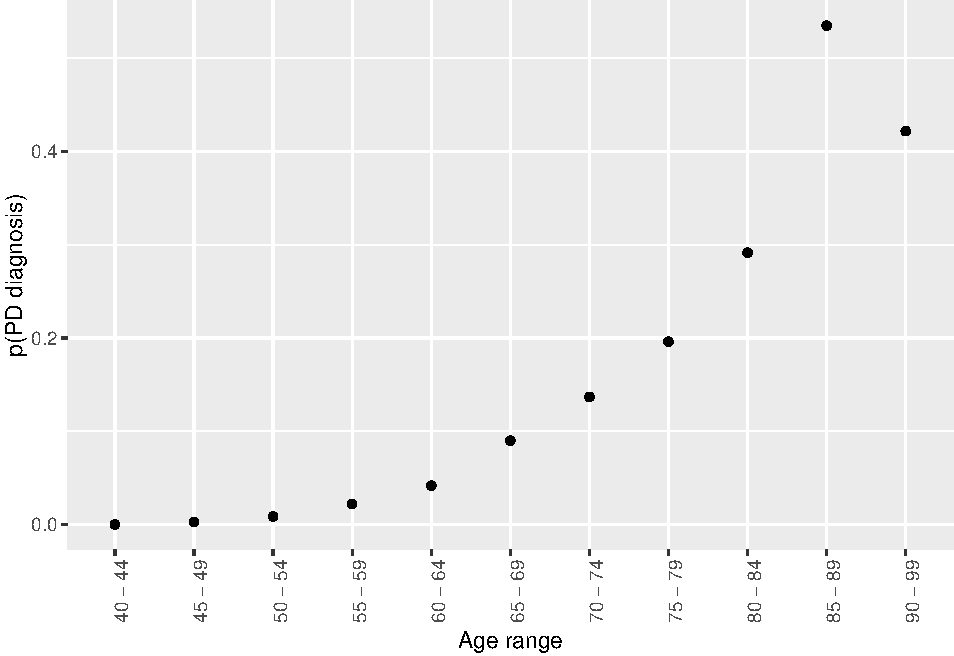
\includegraphics{images/pd_hr-1.pdf}

The distribution of simulated age stratified by PD looks like this:

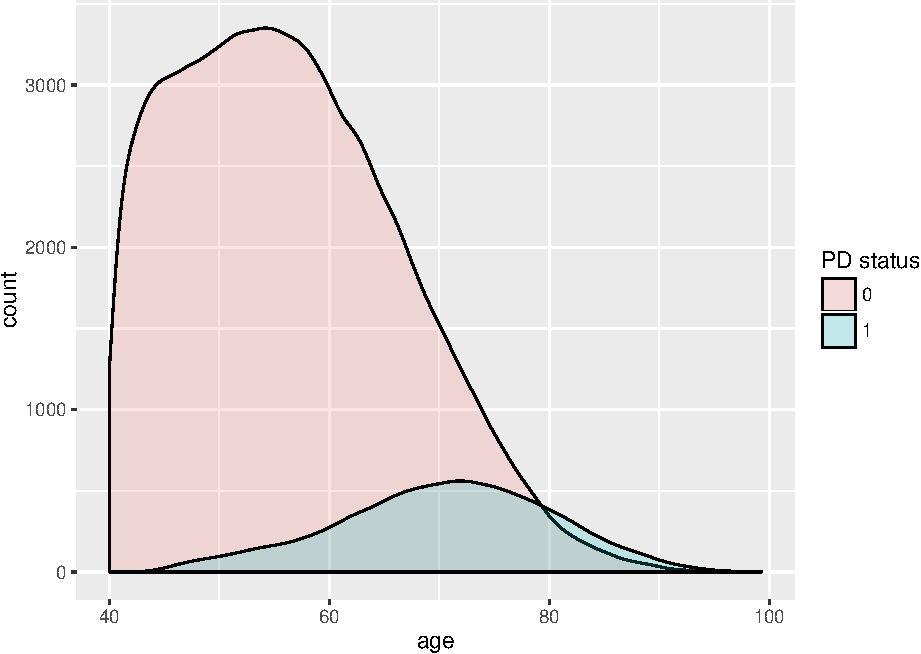
\includegraphics{images/simulated_age_dist-1.pdf}

\subsubsection{Alive/dead status}\label{alivedead-status}

Alive/dead status was a function of age and BMI values. The baseline
survival function was generated from the Gompertz-Makeham law of
mortality, with age related hazard function

\[
h(t) = a \exp(bt) + \lambda
\]

which has CDF

\[
F(t) = 1 - \exp(-\lambda t-\frac{a}{b}(e^{b t}-1))
\]

giving the baseline survival function:

\[
S_{b}(t) = 1 - F(t) = -\exp(-\lambda t-\frac{a}{b}(e^{b t}-1))
\]

which looks like this:

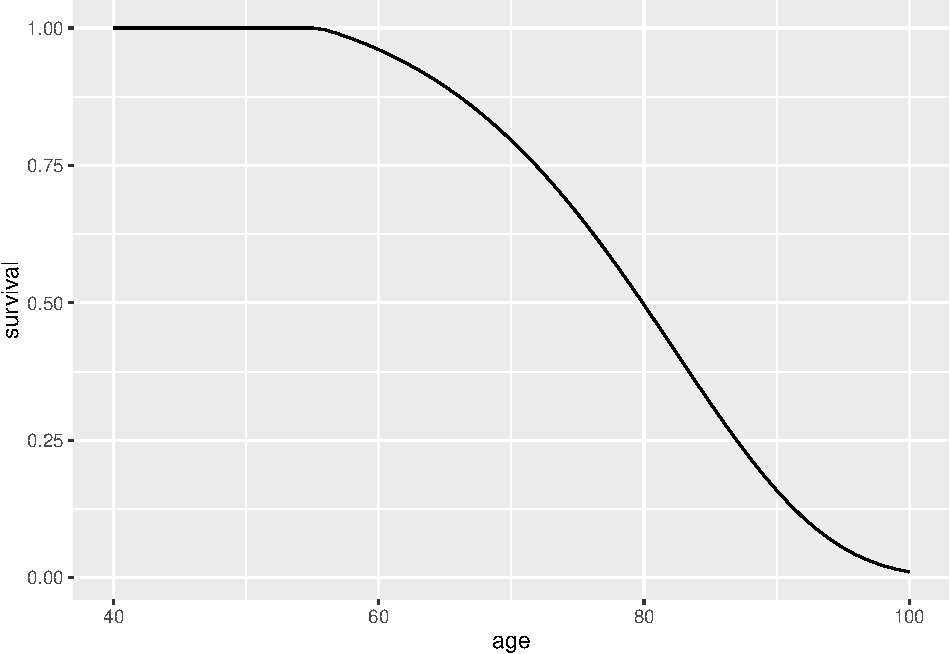
\includegraphics{images/baseline_gm-1.pdf}

The influence of BMI on survival is then incorporated into the full
survival model as

\[
S(t) = S_{b}(t)^{w(x)}
\]

where \(x\) is the BMI value and \(w(x)\) is a function that uses
external data to relate BMI with mortality. A J-shaped relationship
between BMI and hazard ratios ({Berrington de Gonzalez} et al. 2010) was
simulated:

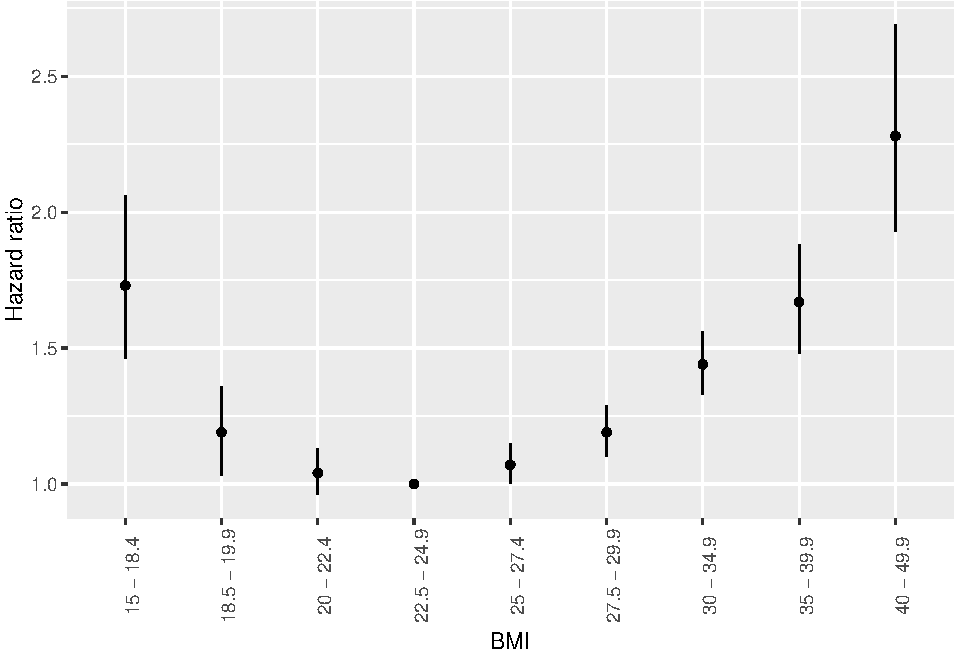
\includegraphics{images/bmi_hr-1.pdf}

The influence of BMI on the survival function is shown here, where the
curves are the survival functions of quartiles of BMI values:

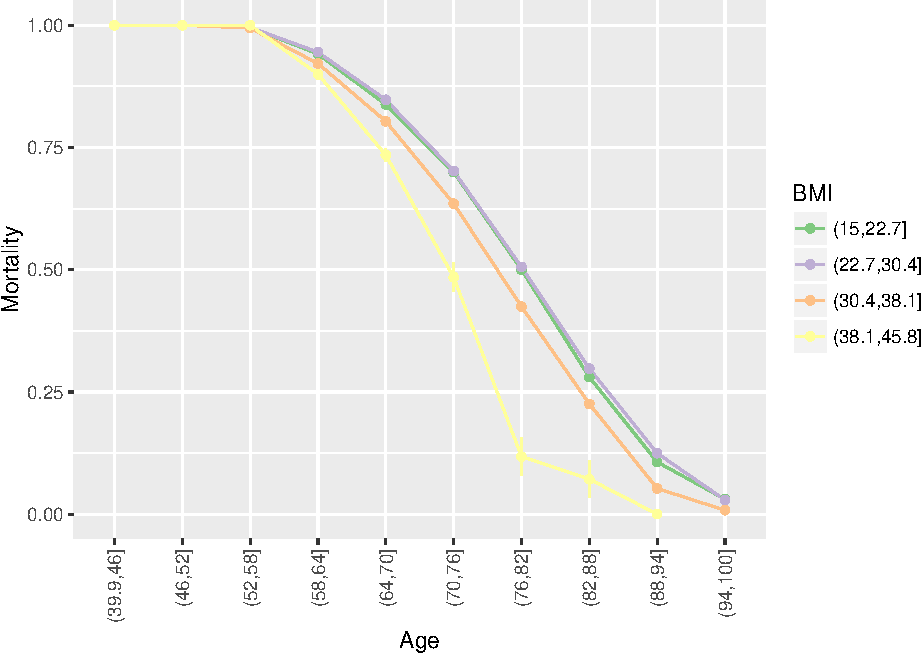
\includegraphics{images/plot_sim_mort_age_bmi-1.pdf}

\subsection{MR analysis of simulated
data}\label{mr-analysis-of-simulated-data}

Perform an MR analysis of BMI on PD in the simulated data. A sample of
108990 are randomly sampled from the individuals who have \texttt{alive}
status to match the sample size and relative numbers of cases and
controls in the PD GWAS (M. A. Nalls et al. 2014). With these simulated
data the following tests can be performed:

\begin{enumerate}
\def\labelenumi{\arabic{enumi}.}
\itemsep1pt\parskip0pt\parsep0pt
\item
  Observational association between BMI and PD
\item
  Two stage least squares estimate of BMI on PD
\item
  Two sample MR using the BMI effect sizes (Locke et al. 2015) and the
  estimated association between these 66 simulated SNPs and the
  simulated PD status. The inverse variance weighting and the MR Egger
  methods are shown here.
\end{enumerate}

An example of what the result looks like for one simulation is shown
here:

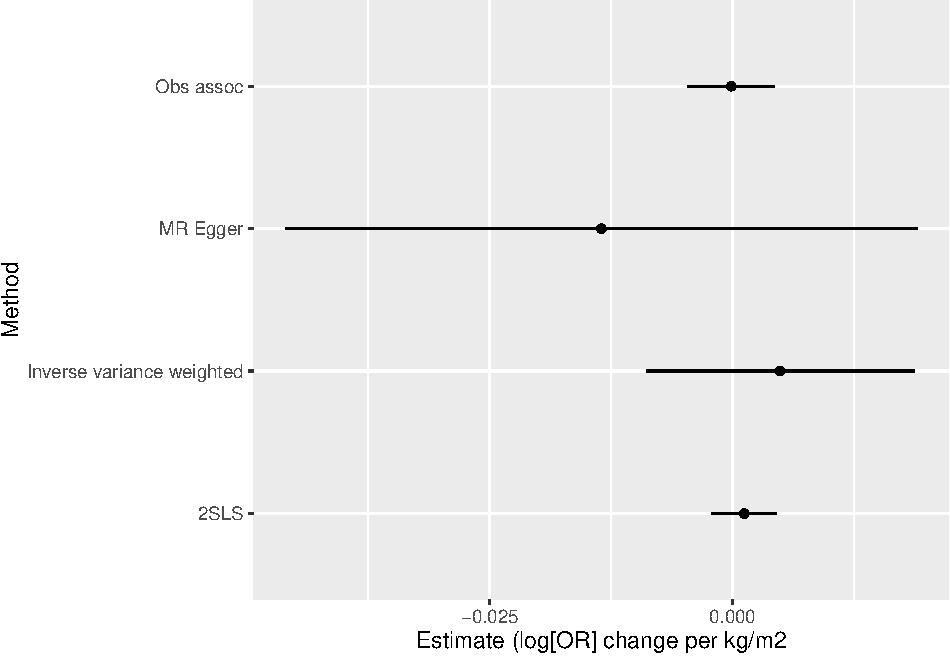
\includegraphics{images/example_mr-1.pdf}

Performing the simulation 1000 times allows us to obtain an empirical
distribution of these estimates under the null model that BMI is not
biologically linked with PD. The results from these simulations look
like this:

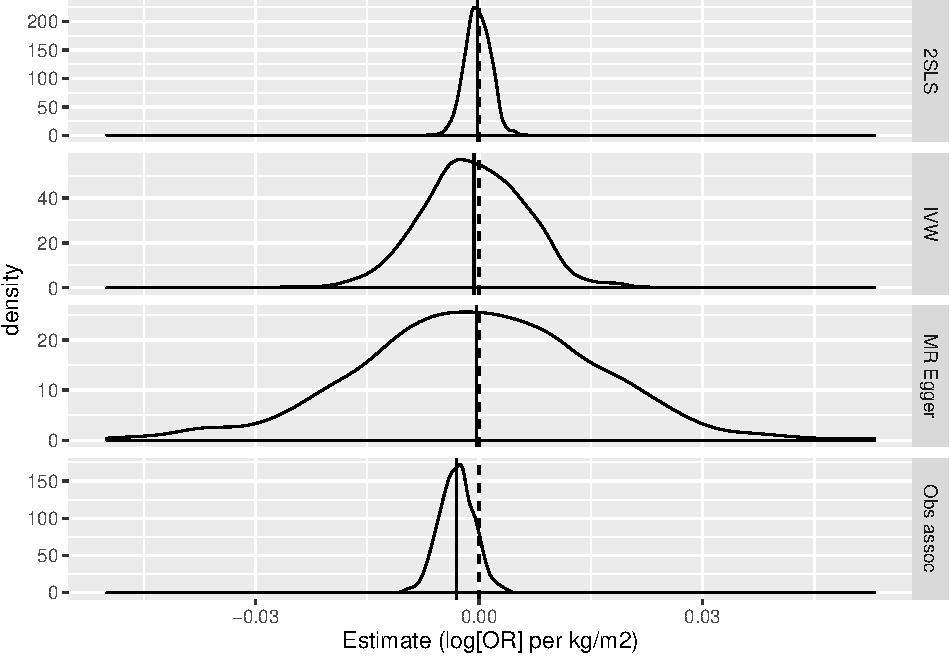
\includegraphics{images/method_comparisons_model1-1.pdf}

So for each of the methods (observational association, 2SLS and 2 sample
MR) there is evidence that survival bias induces an apparent protective
association of BMI on PD. How does this effect relate to those effects
that were estimated in the real data?

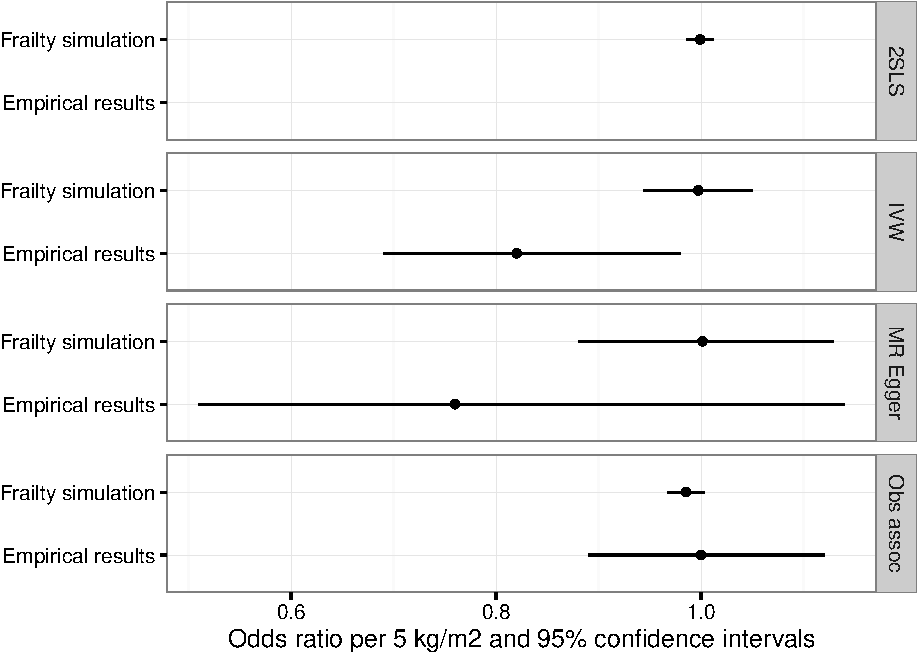
\includegraphics{images/empirical_results-1.pdf}

\textbf{It is clear from this figure that the estimates obtained from
the real data are substantially larger than an effect that would be
induced spuriously from a frailty effect alone.}

\subsection{Limitations}\label{limitations}

The simulations rely on external data to provide hazard ratios for BMI
and incidence rates for PD. The results are unlikely to be grossly
effected by small fluctuations in these estimates.

The frailty simulations allow us to compare the induced associations
using three different methods - observational associations, 2SLS, and 2
sample MR. The distribution of estimates from these three methods are
not consistent. As an example to illustrate this more clearly, a second
simulation was performed using a different hazard model for BMI. Here, a
simple and extreme model was used whereby the HR for BMI on mortality
was 1 for BMI values less than 27, and 5 for BMI values greater than or
equal to 27. The comparison of simulation results from model 1 (J-shaped
model described above) and model 2 (extreme) are shown below:

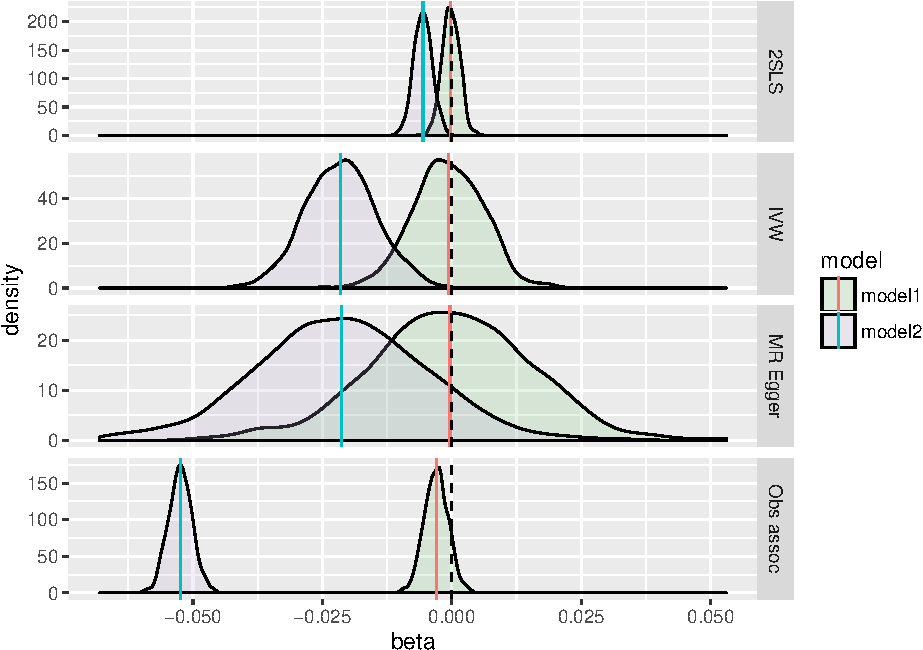
\includegraphics{images/method_comparisons-1.pdf}

As expected model 2 induces a much larger apparent protective effect,
but it's not clear why the different methods give quite drastically
different results.

\subsection*{References}\label{references}
\addcontentsline{toc}{subsection}{References}

{Berrington de Gonzalez}, Amy, Patricia Hartge, James R. Cerhan, Alan J.
Flint, Lindsay Hannan, Robert J. MacInnis, Steven C. Moore, et al. 2010.
``Body-Mass Index and Mortality among 1.46 Million White Adults.''
\emph{New England Journal of Medicine} 363 (23): 2211--19.
doi:\href{http://dx.doi.org/10.1056/NEJMoa1000367}{10.1056/NEJMoa1000367}.

Locke, Adam E., Bratati Kahali, Sonja I. Berndt, Anne E. Justice, Tune
H. Pers, Felix R. Day, Corey Powell, et al. 2015. ``Genetic studies of
body mass index yield new insights for obesity biology.'' \emph{Nature}
518 (7538): 197--206.
doi:\href{http://dx.doi.org/10.1038/nature14177}{10.1038/nature14177}.

Nalls, Mike A, Nathan Pankratz, Christina M Lill, Chuong B Do, Dena G
Hernandez, Mohamad Saad, Anita L DeStefano, et al. 2014. ``Large-scale
meta-analysis of genome-wide association data identifies six new risk
loci for Parkinson's disease.'' \emph{Nature Genetics} 46 (9). Nature
Publishing Group: 989--93.
doi:\href{http://dx.doi.org/10.1038/ng.3043}{10.1038/ng.3043}.

\end{document}
